La relation entre Revendeur et TARE est une relation Hyper Text Protocol (HTTP). La relation HTTP exécute une requête en Transmission Control Protocol (TCP) /IP. L'utilisation de TCP oblige d'avoir un système en d'aquittement. Cette relation peut se modéliser comme ceci :
\\[2cm]
\begin{figure}[h]
    \centering
    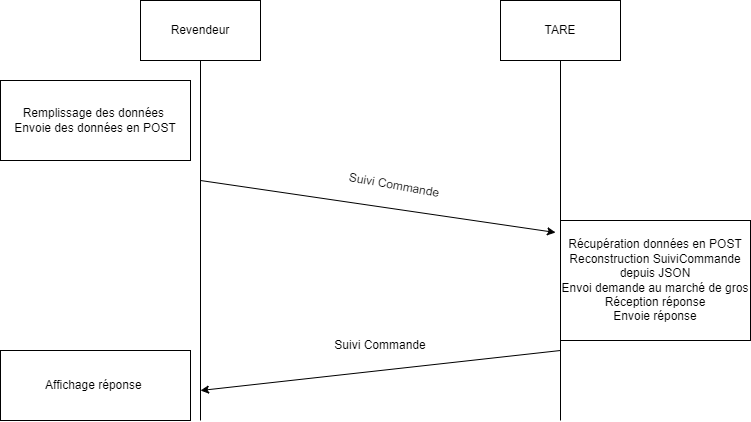
\includegraphics[width=150mm, height=84mm]{images/RevendeurTARE.png}
    \caption{Modélisation de la relation entre Revendeur et TARE}
    \label{img:mesh17}
\end{figure}
\newpage